\chapter{Diagrama de clases}
Un diagrama de clases es un diagrama UML estructural que permite visualizar qué clases componen un proyecto y las relaciones que existen entre ellas. A continución, se muestra el diagrama de clases planteado para el desarrollo del proyecto en curso
\begin{figure}[h!]
	\centering
	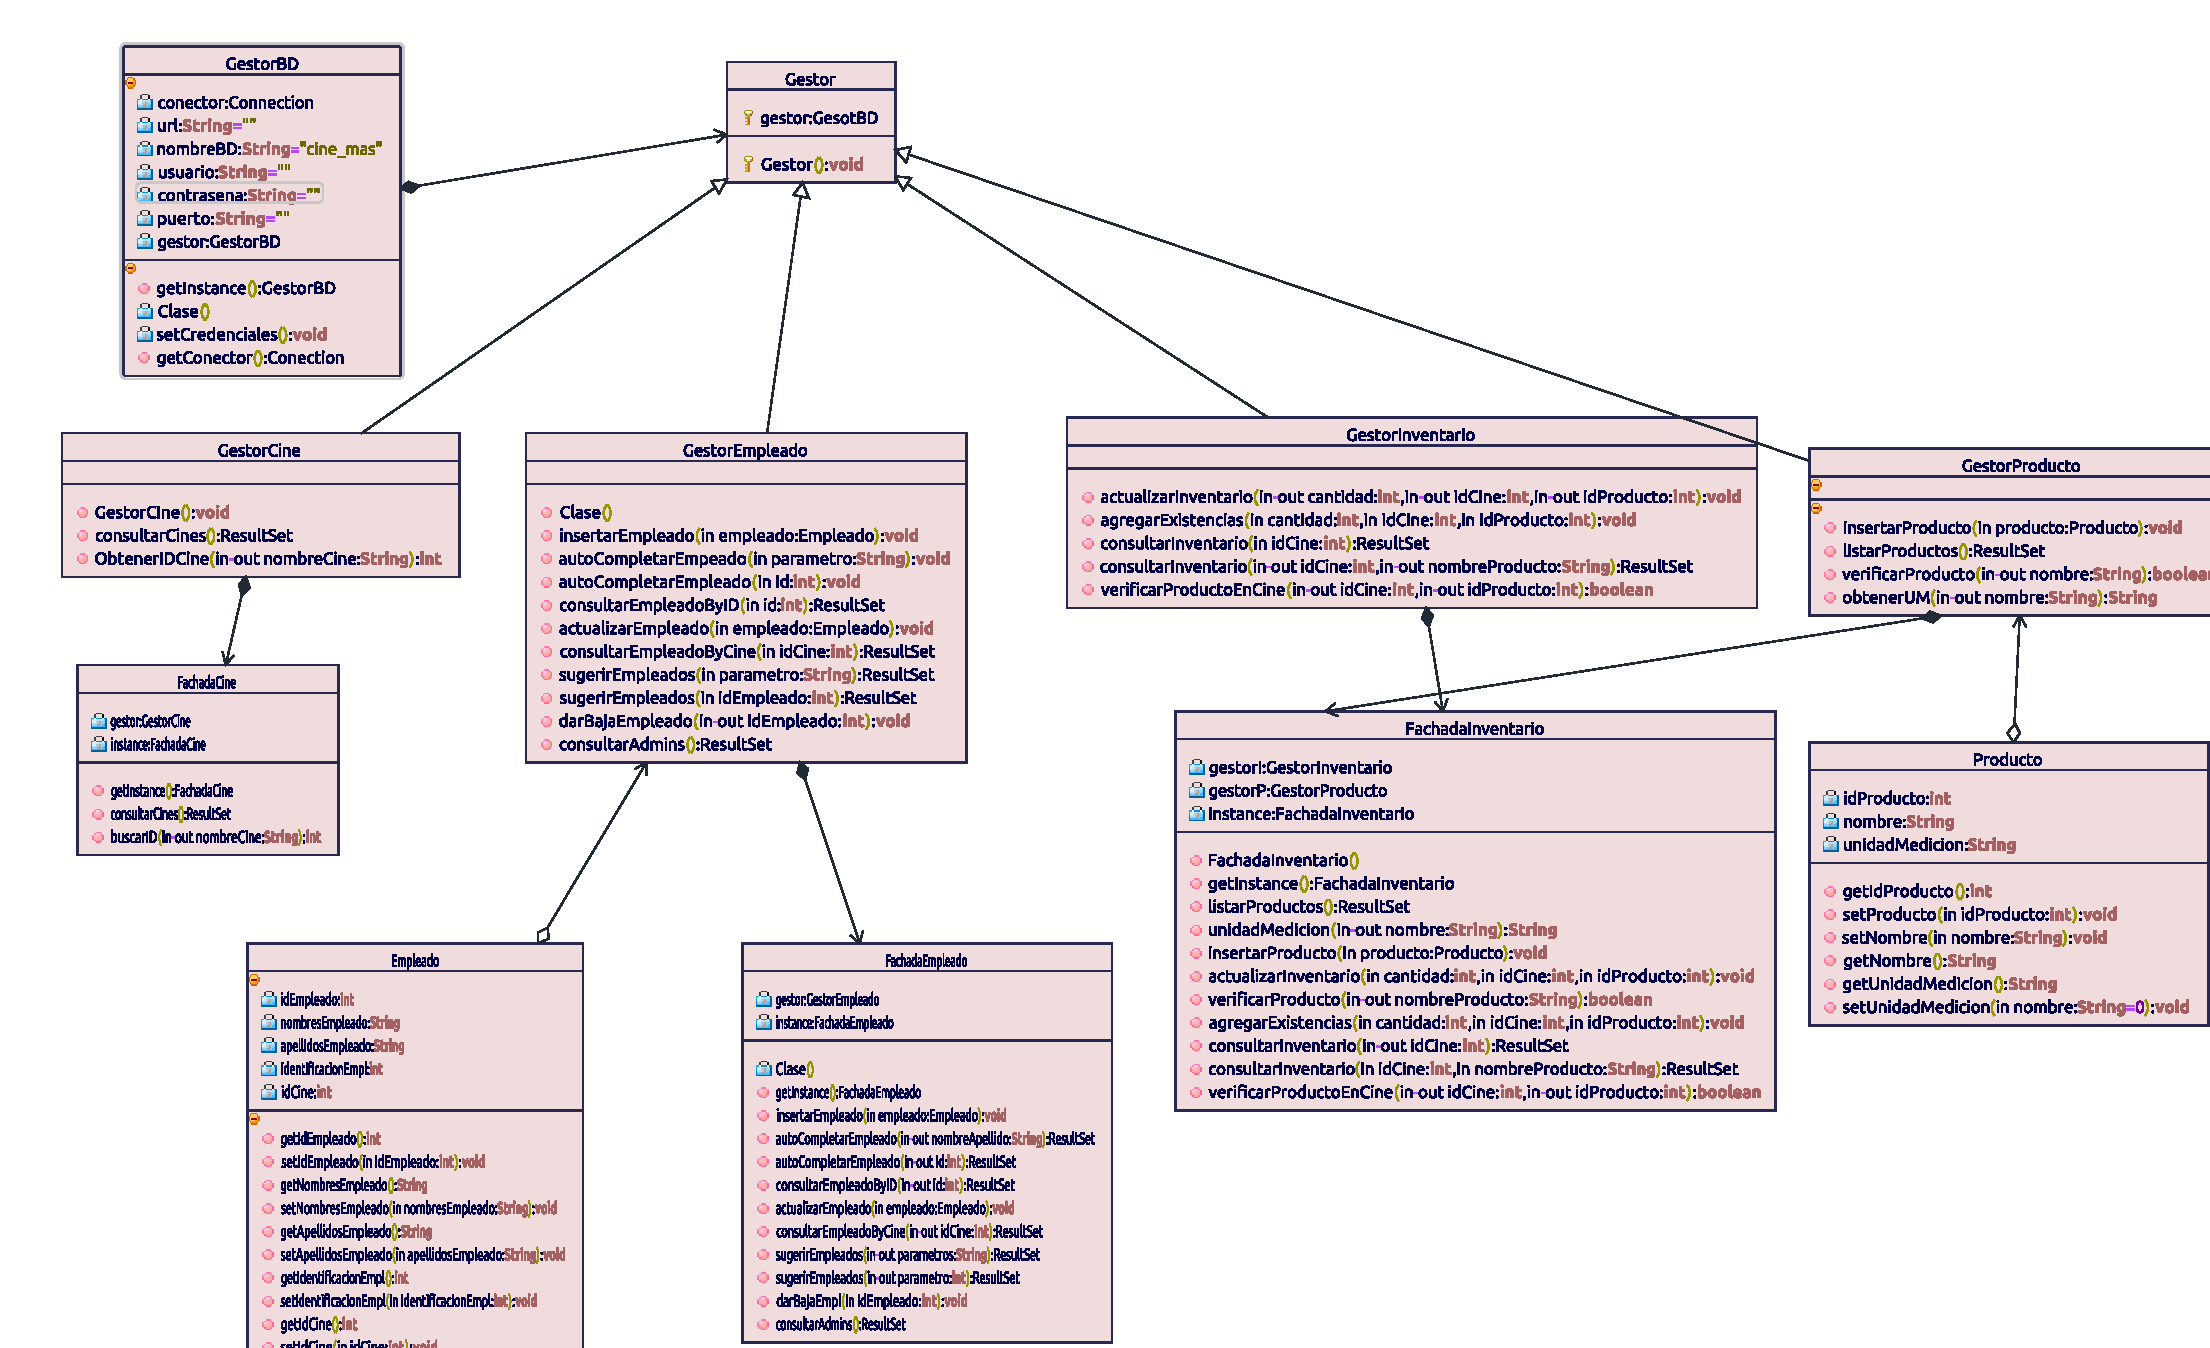
\includegraphics[scale=0.4]{diseno/clases/imgs/clases}
	\caption{Diagrama de clases}
\end{figure}
